A rogue switch such as we developed could be used for numerous disruptions to SDN functionality or attacks that undermine the security assumptions of the system.  We focused our implementation efforts on exploring the possibility of a denial of service (DOS) or distributed denial of service (DDOS) attack on the controller, and discovered its feasibility across multiple controllers.  Based on this result and the basic interactions between controller and switch, we outline several other attacks and disruptions. 

\subsection{DOS on the Controller}
We utilized the basic layer 2 MAC address learning example from the Pox and Ryu controllers with a modifiedhard flow timeout of 1 as our testing setup\footnote{We used l2\_learning as our Pox controller and l2\_switch as our Ryu controller.}. We also utilized the basic mininet setup (a single switch with two hosts) to test the delay caused by our attack on each controller. To test the delay on the controller, we would simply have h1 ping h2. A more complicated controller (e.g. one that does more than simply add the mac address as a flow) would see its performance decrease more significantly than in our example test cases.

 The first attack we attempted was to see if a single switch could overload the controller by rapidly pushing information. We utilized the basic Echo Request (the switch keep-a-live message) as the OpenFlow message to send to the controller to establish a baseline for testing. Bigger packets, particularly ones that require some sort of computation by the controller application, would increase the performance effect on the controller. We started by sending a Echo Request as quickly as possible to the controller without caring about the response. This attack had little effect on the controller and simply resulted in periodic ``TCP Previous Segment Lost" messages as a response from the controller. We believe that the issue with this method was we were never reading in the Echo Replies sent from the controller and the controller was simply ignoring our messages because its send buffer was full. We then modified this attack to send a single Echo Request, wait for an Echo Reply and then instantly send another. This attack caused the controller to continually send Echo Replies but at a controller specified rate - we had to wait for a reply before sending another request. As a result, this attack also had little effect on the controller.

\begin{figure}[ht]
	{\setlength{\fboxsep}{0pt}%
	\setlength{\fboxrule}{1pt}%
	\fbox{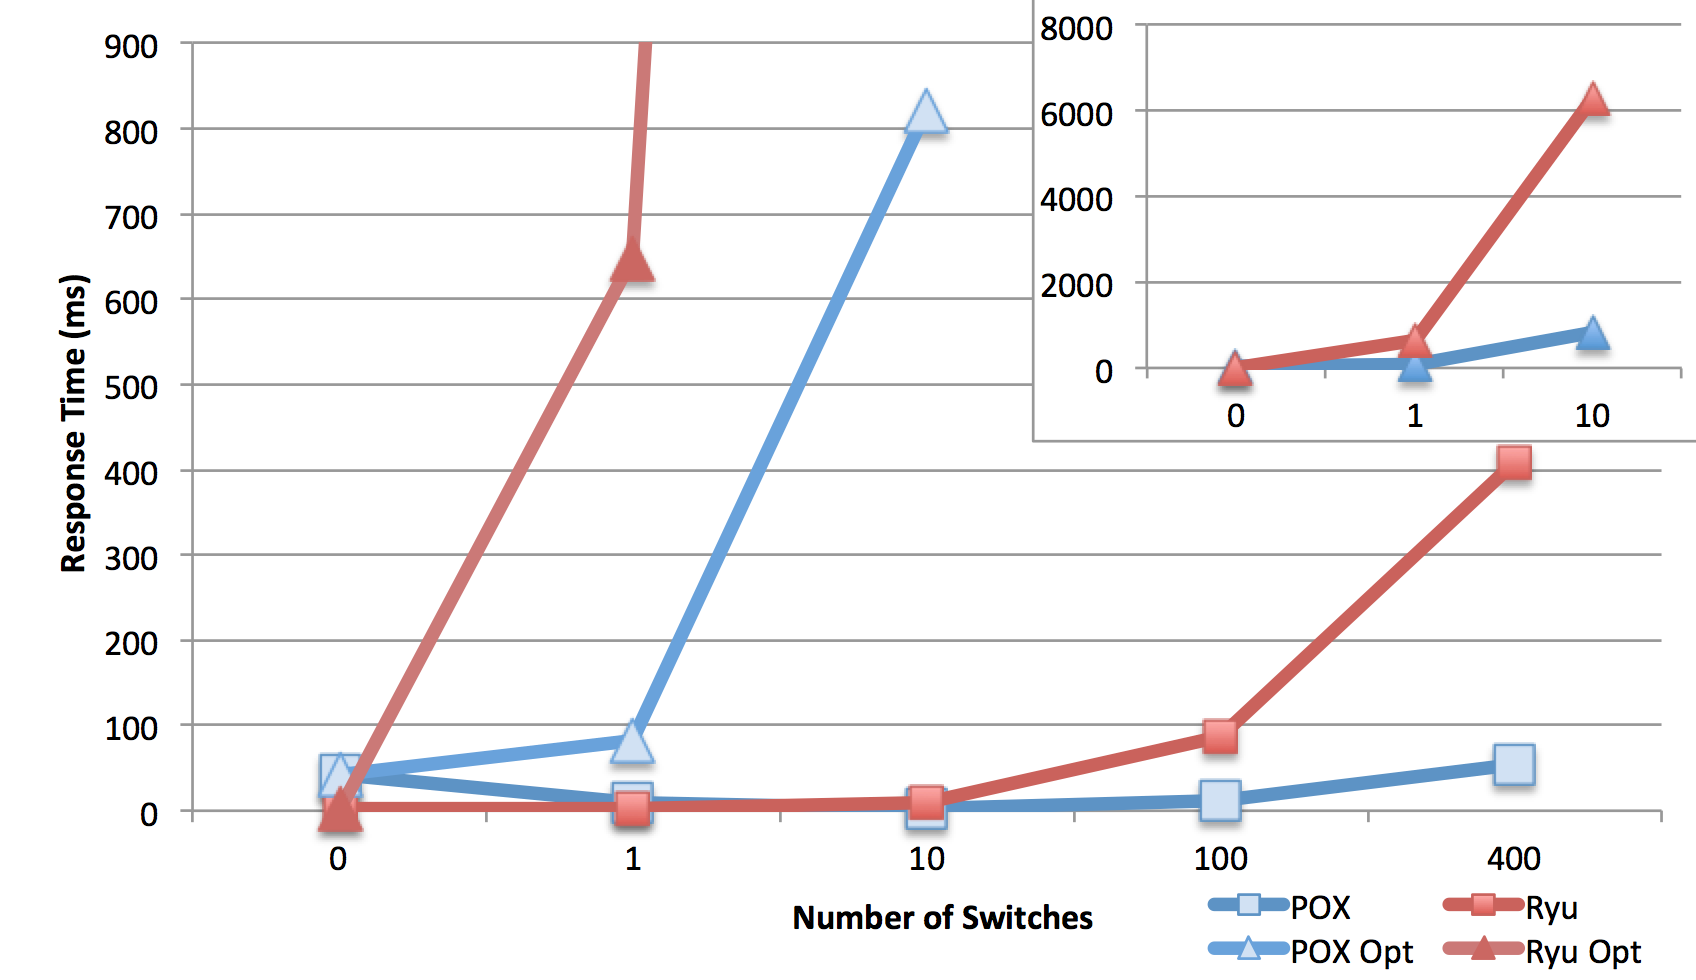
\includegraphics[width=\linewidth]{DOSAttack.png}}
	}%
  \caption{Results of basic and optimized DOS / DDOS on Pox and Ryu Controllers (inset shows expanded view to provide better scale).}
  \label{fig:DOSattacks}
\end{figure}

\subsection{DDoS on the Controller}
   To increase the effect of our attack, we created multiple rogue switches and had each perform the same attack on the controller. Our testing machine was actually the limiting factor in the number of rogue switches we could spawn, but we utilized 400 switches as the max for comparison purposes.  We further optimized our attack by splitting the TCP socket into a distinct listener and sender. We threaded our application so the two actions were not dependent on each other and achieved significantly better results. With our optimized version, we were able to push packets fast enough to cause TCP Window Zero Errors and the controller to drop packets coming from our switch.  These results (shown in Figure \ref{fig:DOSattacks}) show that even a single switch can severely effect the performance of a controller and therefore degrade an entire network. Using just 10 switches with this optimized attack, we were able to produce slowdowns of 779 milliseconds for Pox and 6,305 milliseconds for Ryu.

\subsection{Cloning, Dropping, or Diverting Traffic}

In general, a rogue switch can mishandle packets it receives from the controller or other switches in various ways. Most basically of all, the rogue switch could simply drop packets sent to it, thus creating a service interruption. However, a controller would probably notice this quickly -- it would appear as though the switch had failed, and automated recovery mechanisms would be initiated. More interestingly, a rogue switch could ensure that traffic would be routed through an adversary's middlebox, or could clone traffic and send the cloned stream to the adversary. This would be much more difficult for the controller to detect unless it caused considerable slowdown. This attack could conceivably be used for purposes such as the NSA's MUSCULAR program, which intercepts traffic as it flows between private data centers \cite{muscular}. 


\subsection{Selective Rule Modification}
A rogue switch may behave like a normal switch, leading the controller to believe that it is behaving correctly, but then selectively modifying existing rules, ignoring new Flow Mod requests, or adding new ones. For example, dropping packets will be noticed quickly; but a switch could allow packets to pass through that ought to have been dropped. Because of the difficulty of querying flow table state, the controller may not become aware of this. A compromised switch could thus operate in ``stealth mode" and the inconsistent flow table might only be noticed once the switch allows an attacker to pass through.

The switch could also insert its own modifications; for example, it could add VLAN modification rules in order to have malicious traffic be erroneously treated by other network elements. If normally only packets with a certain VLAN tag are allowed to access a sensitive resource, the switch could ensure that the attacker's traffic appears to have valid permissions.

\subsection{Reporting Falsehoods to the Controller}

A rogue switch can easily send the controller false reports in order to give the controller an incorrect view of the network state. For example, advertising false host attachments is easy; a rogue switch can send the controller Packet-In events with packets which falsely claim to have a particular MAC address as the sender. This could lead the controller to believe that the compromised switch should receive traffic intended for the host. While this would soon lead to packet loss and a noticeable disruption, it would nevertheless allow a switch to eavesdrop when it would not normally be in a position to do so.

Another potential attack is falsifying measurement reports. When a rogue switch receives a Stats Request, it could respond with a modified Stats Reply that selectively hides or distorts information; for example, making overall traffic levels appear lower so as to disguise a DoS attack. 

The rogue switch could also use the controller as a ``relay point" and try to send it Packet In events designed to produce Flow Mods which would then overload other switches' TCAMs or otherwise DoS them. For example, in a MAC learning switch, advertising many new MAC addresses could overload not only the controller, but also other switches, which would have relevant rules installed for the bogus MAC addresses. Thus, instead of attacking each network element individually, the controller gives the attacker an easy, cheap way to concurrently attack many switches at once. 

\subsection{Learning about the Controller}
An adversary could have many reasons to wish to learn more about the controller and the controller's state. By colluding with a rogue switch, the adversary can gain valuable insight into the controller's status.

One possible attack would be for the rogue switch to send Packet In events to the controller and observe the controller's response in order to determine what kind of applications might be running on the controller. This information could be extremely useful for an attacker who wishes to more narrowly target future attacks.

A more passive attack would be for the rogue switch to relay all observed Flow Mod and Send Packet events received from the controller to an adversary. The adversary could then hope to learn about network traffic or other network events by observing patterns in Flow Mods. Certain Flow Mods might indicate that the controller has, for example, detected an intrusion or that a specific host has connected to the network in a certain location. To use the MUSCULAR example again, large companies initiate periodical, large-scale data transfers between data centers; this sort of activity would probably cause very predictable Flow Mod messages to be output from the controller, and thus these could be used to determine when a large data transfer was about to take place. Thus, just knowing what Flow Mods are being issued by the controller could be a source of interesting information for an adversary.

Another possible attack on the SDN Network could be done by exploiting the property of SDN.A Openflow switch in a Software Defined Network is a dumb device that works on basis of rules that are given to it by the controller. Whenever the switch sees a new packet for which a rule has not been defined by the controller the switch simply pushes the packet to the controller and the controller then decides what to do with that new packet. The controller either discards the new packet or pushes a new rule into the flow table of the switch.  
So an attack can be constructed, when the host connected to the rouge switch starts changing its IP Address instantaneously or the host generates packets for which a flow entry is not defined in the flow table of the Openflow switch. The switch will simply forward that packet to the controller and the controller will push a corresponding flow entry to the switch for that new packet. Hence at some point of time the flow table of the switch is expected to overflow and the switch starts to behave abnormally. This attack is possible only when the rate of packets incoming to the switch is greater than the rate at which new flow entries are installed into the openflow switch. In reality the bandwidth between the switch and the controller is just in the order if KBps. So this attack looks possible.    

